\documentclass[a4paper,11pt]{article}

\usepackage{polyglossia}
\setdefaultlanguage{dutch}
%\setdefaultlanguage{english}

\usepackage{fontspec}
%\defaultfontfeatures{Ligatures=TeX} %problem with pyconsole in pythontex
\setmainfont{Latin Modern Roman}
\setsansfont{Latin Modern Sans}[Scale=MatchLowercase]
\setmonofont{Inconsolata}[Scale=MatchLowercase]

\usepackage{amsmath,amssymb}

\usepackage{unicode-math}
\setmathfont[math-style=TeX]{Latin Modern Math}

\usepackage{hyperref}
\usepackage{url}

\usepackage{fancyvrb}
\usepackage{color}
\usepackage{xcolor}

% pythontex: from https://www.youtube.com/watch?v=1AGyBuVCTeE
% to include and evaluate pythoncode in latex document
\usepackage{pythontex}
% matplotlib2tikz prints messages to stdout, so don't include
% stdout automatically; could also redirect stdout to avoid this
\setpythontexworkingdir{.}
% set PythonTeX to use the document root directory as the working
% directory, so that all plots will be saved there; could use 
% another location, but then would need to specify a path when
% using \input and \InputIfFileExists
\usepackage{a4wide}

\usepackage{url}

\usepackage{tikz}
\usetikzlibrary{shapes,arrows,patterns}
\usetikzlibrary{decorations.pathmorphing}
\usetikzlibrary{backgrounds}
\usetikzlibrary{fit}

\usetikzlibrary{shapes.geometric}
\usetikzlibrary{shapes.multipart}
\usetikzlibrary{positioning}
\usetikzlibrary{trees}
\usetikzlibrary{calc}
\usetikzlibrary{graphs}

\tikzset{io/.style={draw=none,minimum width=0mm,minimum height=0mm}}

\tikzset{system/.style={
    draw,rectangle,minimum width=14mm,minimum height=12mm
   }
}
\tikzset{sum/.style={
    draw,circle,minimum size=4mm,minimum width=4mm
   }
}


\renewcommand{\arraystretch}{1.3}

\title{Tutorial UAVREG\\ Baanregeling Quadcopter}
\author{Rufus Fraanje}
\date{17/04/2017}

\begin{document}
\maketitle

\section{Inleiding}
Autopilot systemen zijn inmiddels zeer gangbaar. In vliegtuigen worden
autopilots al geruimte tijd gebruikt. Ook de meeste drones zijn uitgerust met
een autopilot systeem. In sommige gevallen dient de autopilot er slechts voor
om de drone (veilig) terug te laten vliegen naar zijn thuisbasis, in veel
gevallen kan met een autopilot een traject langs van tevoren bepaalde punten
worden gevlogen. 

In deze tutorial ga je zelf een autopilot besturing realiseren waarmee een
quadcopter een traject kan afleggen. Dit zal worden gedaan met behulp van een
aantal PID (proportionele, integrerende en differenti\"erende) regelaars en
nog een aantal rekenkundige bewerkingen. 

De leerdoelen van deze tutorial zijn:
\begin{itemize}
  \item begrijpen hoe de verschillende regelaars samenwerken om de quadcopter
    te besturen en hoe dit ge\"implementeerd kan worden in een Python simulatie;
  \item een PID regelaar kunnen implementeren;
  \item de parameters $K_p$, $K_i$ en $K_d$ van PID regelaars kunnen
    instellen door middel van `tunen'.
\end{itemize}
De autopilot besturing zullen we hier ontwerpen in een simulatie in
Python. Zo kunnen we ervaring opdoen, zonder dat de quadcopter door instabiel
gedrag kapot gaat en
kunnen we de situatie iets vereenvoudigen. In de praktijk is het namelijk vaak lastig
de precieze positie en ori\"entatie van de quadcopter exact te kennen, in deze
simulatie kennen we de positie en ori\"entatie exact. 

Voor de simulatie maken we gebruik van twee Python modules:
\begin{itemize}
  \item \texttt{pybullet}: een module waarmee de beweging van de quadcopter
    berekend kan worden (quadcopter dynamica), \texttt{pybullet} is een
    interface naar de krachtige (C++) bibliotheek \texttt{bullet}
    (\url{http://bulletphysics.org}) die ook wordt gebruikt als physics-engine
    in programma's als Blender en diverse computer games, zie bijvoorbeeld
    \url{https://en.wikipedia.org/wiki/Bullet_(software)}. 
  \item \texttt{pyqtgraph}: een module voor (extreem) snelle visualisatie van 2D
    en 3D graphics, deze module maakt gebruik van OpenGL waarmee direct de
    grafische kaart kan worden aangestuurd (\url{http://www.pyqtgraph.org});
\end{itemize}
De installatie van deze modules wordt uitgelegd in
paragraaf~\ref{sec:install}. Het principe van de autopilot wordt aan de hand
van een blokdiagram uitgelegd in paragraaf~\ref{sec:regeling}. 
Met behulp van de modules \texttt{pybullet} en \texttt{pyqtgraph} is een deel van de simulatie al
geprogrammeerd, hoe dit is gedaan wordt uitgelegd in
paragraaf~\ref{sec:implementatie}.
De opdracht voor de tutorial vind je in paragraaf~\ref{sec:opdracht}.

\section{Benodigde Python modules}
\label{sec:install}
\subsection{\texttt{pybullet}}
The module \texttt{pybullet} kan worden aangemaakt door de \texttt{bullet}
bibliotheek te compileren. Dit kan vrij eenvoudig via het \texttt{pip install
<name\_of\_package>} commando. Hiervoor heb je, onder Windows, echter ook
Microsoft Visual C++ 14.0, met de Build Tools 2015 (niet 2017!). Dit gaat
alsvolgt:
\begin{itemize}
\item Download de Python distributie Anaconda3 van \url{https://www.continuum.io/downloads}.

\item Ga met de verkenner naar \texttt{.\backslash Anaconda3\backslash
  Scripts\backslash spyder.exe} en maak een snelkoppeling naar je desktop.

\item Wijzig in de eigenschappen van de snelkoppeling de titel en het ikoon:
  kies \texttt{.\backslash Anaconda3\backslash Scripts\backslash spyder.ico}. Wacht nog even met opstarten van Spyder.

\item Microsoft Visual C++ 14.0 is nodig. Haal het op bij "Microsoft Visual C++ Build Tools 2015": 
\url{http://landinghub.visualstudio.com/visual-cpp-build-tools}. Let op dat je versie 14.0 kiest van MS-VS 2015 en niet 2017!

\item Herstart je laptop.

\item Open een command window met \texttt{cmd} en ga naar \texttt{.\backslash Anaconda3\backslash Scripts} met het commando \texttt{cd} (change directory). Dit omdat je misschien nog een oude versie van Python geïnstalleerd hebt staan.

\item Run in de command window: \texttt{pip install pybullet} en daarna (de volgende stappen zijn niet nodig voor \texttt{pybullet} maar wel voor deze tutorial, en komen in de volgende paragraaf ook nog aan bod, als je ze nu al ge\"installeerd hoef je dat straks niet nog een keer te doen):

\item \texttt{pip install PyOpenGL}

\item \texttt{pip install PyOpenGL\_accelerate}

\item \texttt{pip install pyqtgraph}

\item \texttt{pip install trimesh}

\end{itemize}
Test of de module goed wordt ingelezen met \texttt{import}:
\begin{pyconsole}
import pybullet
dir(pybullet)

\end{pyconsole}
Werp eventueel een blik op de help met \texttt{help(pybullet)}. Uitgebreide
documentatie vind je in 
\url{https://docs.google.com/document/d/10sXEhzFRSnvFcl3XxNGhnD4N2SedqwdAvK3dsihxVUA/edit?usp=sharing}
maar voor deze tutorial is het niet nodig deze door te werken.

Voor de quadcopter simulatie hebben we ook de volgende bestanden, beschikbaar via Blackboard, nodig:
\begin{itemize}
\item \texttt{plane.urdf} en \texttt{plane.obj}
\item \texttt{quadrotor.urdf} en \texttt{quadrotor\_base.obj}
\end{itemize}
De \texttt{urdf} bestanden zijn Universal Robot Description Format bestanden die objecten in een 3D wereld specificeren, zoals vorm en afmetingen, massa en traagheidsmoment. Het \texttt{urdf}-formaat is oorspronkelijk ontwikkeld voor het Robot Operating System (ROS) \cite{ros}, maar wordt nu ook breder gebruikt. The \texttt{obj}-bestanden bevatten een mesh-beschrijving afkomstig van een 3D CAD programma, die wordt gebruikt in de \texttt{urdf}-bestanden.

De \texttt{bullet} bibliotheek heeft ook een visualisatie-mogelijkheid. Deze
zullen we in het vervolg niet gebruiken, maar je kunt hiermee wel alvast
controleren of het grondvlak (\texttt{plane.urdf}) en de quadcopter
(\texttt{quadrotor.urdf}) goed weergegeven worden:
\begin{pyconsole}
import pybullet as p
#choose connection method: GUI, DIRECT, SHARED_MEMORY
p.connect(p.GUI)
p.loadURDF("plane.urdf",0,0,-1)
#load URDF, given a relative or absolute file+path
quadcopterId = p.loadURDF("quadrotor.urdf")

\end{pyconsole}
Om een idee te geven wat je met \texttt{pybullet} kunt doen, laten we gedurende
een fractie van een seconde een verticale kracht van 100 N (vector [0,0,100]) uitoefenen in het
centrum van de quadcopter (positie [0,0,0]), en vervolgens 100 simulatiestappen uitvoeren. Dat
kun je doen met de volgende code in Python (voer deze commando's uit op de
Python command-line): 
\begin{pyconsole}
#give a vertical impulsive force of 100 N at center of quadcopter
p.applyExternalForce(quadcopterId,-1,[0,0,100],[0,0,0],p.LINK_FRAME)
#do a 100 time-steps in the simulation to see the effect of the force impulse 
for _ in range(100): p.stepSimulation()
#note we use _ here rather then a letter such as i, this is a habit in python
#to represent a dummy parameter, that's not being used anymore

\end{pyconsole}
Experimenteer een beetje, bijvoorbeeld door te kijken wat er gebeurd
als je nog meer \texttt{p.stepSimulation()} commando's uitvoert. Ook kun
je eens proberen een kracht in een andere richting of op een ander punt op de
quadcopter uit te oefenen of door gravitatie toe te voegen met \sloppy 
\texttt{p.setGravity(0,0,-9.8)}. Voor sommige simulatie experimenten is het
handig om de gravity vector gelijk aan 0 te maken, dat kan dus eenvoudig met
\texttt{p.setGravity(0,0,0)}. De optie \texttt{p.LINK\_FRAME} geeft aan dat de
kracht wordt uitgeoefend op de positie in het assenstelsel gekoppeld aan het
quadcopter object. Een alternatief is de optie \texttt{p.WORLD\_FRAME}, waarbij
de kracht wordt uitgeoefend op de positie in het assenstelsel van de vaste
wereld (dit zullen we bij de quadcopter echter niet doen).

Maar zoals gezegd, zullen we niet gebruikmaken van de ingebouwde visualisatie
in \texttt{bullet} en \texttt{pybullet}, aangezien deze nogal wat CPU-power
vraagt en minder snel is dan \texttt{pyqtgraph}. Sluit dus het venster met het
grondvlak en de quadcopter en ga verder met het installeren van
\texttt{pyqtgraph}.

\subsection{\texttt{pyqtgraph}}
Voor het plotten van 2D en 3D grafieken heb je wellicht al gebruik gemaakt van
de module \texttt{matplotlib}. Deze module is uitstekend voor het maken van
allerlei grafieken (zie de \texttt{matplotlib}-gallery) maar minder geschikt
voor `real-time' visualisatie, omdat \texttt{matplotlib} hiervoor niet snel
genoeg is. De module \texttt{pyqtgraph} is hiervoor beter geschikt, aangezien
deze direct de grafische kaart kan aansturen met OpenGL en daardoor extreem
snel is. Het installeren van \texttt{pyqtgraph} gaat het makkelijkst via het
commando \sloppy \texttt{pip install <python\_module\_naam>} (zoals hierboven ook al gedaan). We hebben in
totaal vier extra modules nodig, die niet standaard in de Anaconda distributie
van Python ge\"installeerd zijn, dat zijn de modules \texttt{PyOpenGL},
\texttt{PyOpenGL\_accelerate}, \texttt{pyqtgraph} en
\texttt{trimesh}\footnote{We hebben daarnaast ook de \texttt{math} module
  nodig die behoord tot de standaard library van Python en de \texttt{numpy}
module, waarvan we aannemen dat deze ook reeds ge\"installeerd is. In de
Anaconda distributie komt \texttt{numpy} standaard mee. Als \texttt{numpy}
niet ge\"installeerd is, kan dat eenvoudig door middel van bijvoorbeeld het
commando \texttt{pip install numpy}.} De module \texttt{trimesh} hebben we nodig om de CAD beschrijvingen in de \texttt{obj}-bestanden om te zetten naar een mesh-structuur  van driehoekjes die door \texttt{pyqtgraph} gevisualiseerd kan worden. Het installeren gaat alsvolgt. Open onder Windows een Windows Command Prompt Window en geef daarin het commando:
\begin{verbatim}
C:\ pip install PyOpenGL PyOpenGL_accelerate pyqtgraph trimesh
\end{verbatim} 
Onder Linux of Mac OSX open je een terminal en geef je voor user-niveau installatie het commando
\begin{verbatim}
$ pip install PyOpenGL PyOpenGL_accelerate pyqtgraph trimesh
\end{verbatim} 
en voor installatie op system-wide niveau het commando 
\begin{verbatim}
$ sudo -H pip install PyOpenGL PyOpenGL_accelerate pyqtgraph trimesh
\end{verbatim} 
Test of \texttt{pyqtgraph} goed is ge\"installeerd door enkele voorbeelden die met \texttt{pyqtgraph} meekomen uit te proberen, door middel van:
\begin{pyconsole}
from pyqtgraph import examples
examples.run()

\end{pyconsole}
Om \'e\'en of andere reden werkt \texttt{examples.run()} soms niet. In dat
geval kun je de \texttt{pyqtgraph} voorbeelden ook starten vanuit de windows
command line met het commando:
\begin{verbatim}
C:\ python -m pyqtgraph.examples
\end{verbatim}
Als het goed is zie je nu een menu met verschillende voorbeelden. Probeer in elk geval het voorbeeld \texttt{Basic Plotting} en onder 3D Graphics het voorbeeld \texttt{Mesh}. Bij het \texttt{Mesh} voorbeeld moet er een venster met een aantal 3D objecten verschijnen.

Het is handig om even na te gaan hoe je met de muis het beeld kan verschuiven, roteren en in- en uitzoomen. Uit de documentatie van \texttt{pyqtgraph}, zie \url{http://www.pyqtgraph.org/documentation/mouse_interaction.html}, halen we de volgende regels: 
\begin{verbatim}
3D visualizations use the following mouse interaction:
  • Left button drag: Rotates the scene around a central point
  • Middle button drag: Pan the scene by moving the central “look-at” point
    within the x-y plane
  • Middle button drag + CTRL: Pan the scene by moving the central “look-at”
    point along the z axis
  • Wheel spin: zoom in/out
  • Wheel + CTRL: change field-of-view angle
And keyboard controls:
  • Arrow keys rotate around central point, just like dragging the left mouse button
\end{verbatim}

Om met de muis het beeld te kunnen aanpassen en het beeld voortdurend te
verversen is het nodig de GUI event loop voor \texttt{pyqtgraph} te starten.
In de voorbeelden wordt dit gedaan door middel van een paar commando's. Wij
zullen dat doen door de GUI event loop van tevoren te starten. Als je gebruik
maakt van Spyder kan dat eenvoudig op de volgende manier (hoef je maar \'e\'en
keer te doen):
\begin{quote}
  Ga naar het \texttt{Tools} menu, kies \texttt{Preferences}, kies vervolgens
  \texttt{IPython console}, selecteer de \texttt{Graphics tab}, en kies dan
  vervolgens als \texttt{Graphics backend} de keuze \texttt{Qt5} backend.
\end{quote}
Zorg er vervolgens voor dat je de \texttt{ipython} console gebruikt als Python
interpreter (dit is standaard in Spyder, maar gebruik dus niet de python
console). Als je de \texttt{ipython} console gebruikt, ziet de command prompt
er als volgt uit (of vergelijkbaar):
\begin{verbatim}
Python 3.5.2 (default, Nov 17 2016, 17:05:23) 
Type "copyright", "credits" or "license" for more information.

IPython 5.1.0 -- An enhanced Interactive Python.
?         -> Introduction and overview of IPython's features.
%quickref -> Quick reference.
help      -> Python's own help system.
object?   -> Details about 'object', use 'object??' for extra details.

In [1]: 
\end{verbatim}
De \texttt{ipython} console heeft een groot aantal handige opties. Probeer bijvoorbeeld eens de volgende commando's om de huidige folder en de inhoud daarvan te bekijken:
\begin{verbatim}
In [1]: pwd
In [2]: ls
\end{verbatim}
Heel soms werkt de \texttt{<Enter>} toets in \texttt{ipython} niet naar behoren. In dat geval maak gebruik van \texttt{<Shift><Enter>} in plaats van \texttt{<Enter>}. 
Ook handig is het commando \texttt{cd}, waarmee  je  naar een andere folder kan gaan (vergelijkbaar met het Linux terminal-commando \texttt{cd}).

De GUI event loop kun je ook starten vanuit de \texttt{ipython} console, dat gaat met de \texttt{gui} magic\footnote{Magics zijn uitbreidingen van de python commando's in \texttt{ipython}. Een andere handige magic is de \texttt{run} magic, waarmee python-scripts uitgevoerd kunnen worden. Voor meer informatie over magics raadpleeg de \texttt{quickref} magic.}, geef daarvoor het volgende commando (raadpleeg eventueel ook de help met \texttt{\%gui?}):
\begin{verbatim}
In [3]: %gui qt5      # comment: sommige oudere python versies gebruiken
                      # qt4 ipv qt5, in dat geval geef de optie qt of qt4
In [4]: %gui?
\end{verbatim}
Echter op deze manier blijft de instelling niet behouden, dus je kunt beter de instelling via de \texttt{Preferences} onder het \texttt{Tools} menu maken.

Je zult soms de Python kernel van de  \texttt{ipython} console opnieuw willen starten. Dat kun je eenvoudig doen met de toets-combinatie \texttt{<Ctrl>.} (dus de control-toets en de punt-toets tegelijk indrukken).

\section{Quadcopter regeling}
\label{sec:regeling}

\subsection{Vrijheidsgraden van de quadcopter}
Voordat we daadwerkelijk beginnen met de quadcopter simulatie, laten we eerst naar de principes van de quadcopter autopilot besturing kijken. Er zijn verschillende mogelijkheden, maar wij zullen gebruik maken van een schema gebaseerd op een aantal PID (proportionele, integrerende en differenti\"erende) regelaars, voor elke vrijheidsgraad \'e\'en. Dus in totaal hebben we zes PID regelaars, \'e\'en voor de $x$-richting, \'e\'en voor de $y$-richting, 
\'e\'en voor de $z$-richting, \'e\'en voor de roll, \'e\'en voor de pitch, en \'e\'en voor de yaw.  De roll, pitch en yaw vrijheidsgraden zijn rotaties om respectievelijk de $x$, de $y$ en de $z$ as van het assenstelsel dat vast gekoppeld is aan de quadcopter (locaal assenstelsel). De roll, pitch en yaw worden ook wel de $XYZ$ Euler hoeken genoemd.

De quadcopter heeft echter maar vier motoren, die onafhankelijk kunnen worden aangestuurd. Dat betekent dat we op elk moment maar vier vrijheidsgraden kunnen besturen, dat zijn:
\begin{itemize}
\item \textbf{thrust}, som van de krachten van de motoren, levert versnelling loodrecht op het vlak van de quadcopter;
\item \textbf{roll}, moment om de $x$-as van de quadcopter, veroorzaakt door het koppel van de twee motoren langs de $y$-as, levert een hoek-versnelling om de $x$-as van de quadcopter;
\item \textbf{pitch}, moment om de $y$-as van de quadcopter, veroorzaakt door het koppel van de twee motoren langs de $x$-as, levert een hoek-versnelling om de $y$-as van de quadcopter;
\item \textbf{yaw}, moment om de $z$-as van de quadcopter, veroorzaakt door som van de momenten van de vier motoren, levert een hoek-versnelling om de $z$-as van de quadcopter.
\end{itemize}

Als de quadcopter niet gekanteld is, ofwel geen roll en pitch maakt, en dus de verticale $z$-as die vast zit aan de quadcopter parallel staat
met de $z$-as van de vaste-wereld, dan kunnen we met de \textbf{thrust}
de hoogte regelen. Dit wordt behandeld in de volgende paragraaf.

 Daarna zullen we de algemene situatie behandelen, waarin we eerst
 een kracht-vector berekenen met de PID regelaars voor positie in de
 vaste-wereld, en vervolgens de quadcopter kantelen zodat de quadcopter
 loodrecht op deze kracht-vector komt te staan. Deze krachtvector kan dan dus gerealiseerd worden door de juiste hoeveelheid thrust uit te oefenen.

Om de autopilot niet te complex te maken, zullen we de yaw-regeling  buiten beschouwing laten, ofwel de yaw zal constant op 0 rad geregeld worden\footnote{De yaw moet wel gestabiliseerd worden, omdat de quadcopter uit zichzelf instabiel is. Ofwel, een zeer gering moment in de yaw-richting leidt al tot het weglopen van de yaw, waardoor deze niet meer constant op 0 rad staat.}.

Vanaf nu, zullen we ook aannemen dat de vier motoren alleen een kracht uitoefenen. We laten dus airodynamische aspecten en de toerentalregeling buiten beschouwing. Dit is een benadering, waardoor de autopilot niet \'e\'en op \'e\'en naar de praktijk overgezet kan worden. De principes achter de PID regelingen zijn echter ook in de praktijk zeer goed bruikbaar.

\subsection{Hoogte regeling}
Bij de regeling van de hoogte laten we de overige vijf vrijheidsgraden buiten beschouwing en nemen we aan dat de quadcopter horizontaal staat. Figuur~\ref{fig:blokschema_hoogte} geeft het blokschema van de hoogte regeling, waarbij de referentiewaarde $r_z$ de gewenste hoogte is, $z$ de daadwerkelijke hoogte van de quadcopter, $e_z$ de regelfout, $F$ de regelkracht berekend door de PID regelaar, $F_{z,comp}$ is een compensatie term in de besturing waarmee de zwaartekracht gecompenseerd kan worden en tot slot $F_z=-mg$ is de zwaartekracht. Merk op, dat we voor zowel de krachten als de positie de vertikale richting omhoog de positieve richting is. Merk ook op, dat alle signalen, met uitzondering van $F_z$, afhangen van de tijd. Het is dus eigenlijk $r_z(t)$ in plaats van $r_z$, beide notaties zullen we gebruiken.
\begin{figure}
\centering
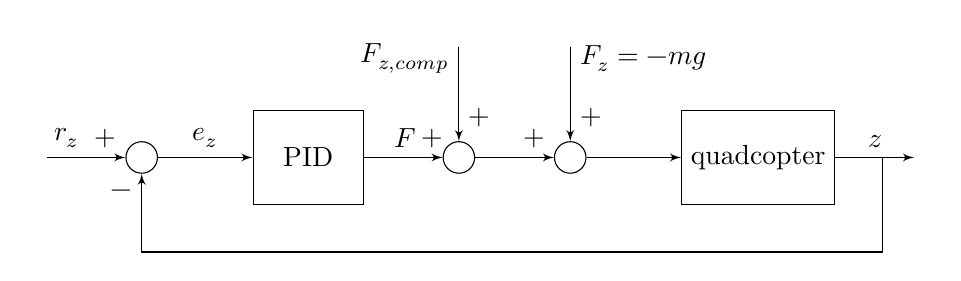
\begin{tikzpicture}[node distance=12mm,>=latex']
	\node[io] (ref) {};
	\node[sum,right=1cm of ref] (sum1) {};
    \node[system,right=of sum1] (pid1) {{PID}};
	\node[sum,right=1cm of pid1] (sum2) {};
	\node[sum,right=1cm of sum2] (sum3) {};
	\node[system,right=of sum3] (quadcopter) {quadcopter};
	\node[io,above=of sum2] (fzcomp) {};
	\node[io,above=of sum3] (fz) {};
    \node[io,right=1cm of quadcopter] (pos) {};

    \draw[->] (ref)  -- node[near start,above] {$r_z$} node[near end,above] {$+$} (sum1);
    \draw[->] (sum1) -- node[above] {$e_z$} (pid1);
    \draw[->] (pid1) -- node[above] {$F$} node[above,very near end] {$+$} (sum2);
	\draw[->] (fzcomp) -- node[very near start,left]{$F_{z,comp}$} node[right,near end] {$+$} (sum2);
	\draw[->] (fz) -- node[very near start,right]{$F_{z}=-mg$} node[right,near end] {$+$} (sum3);
	\draw[->] (sum2) -- node[above,near end] {$+$} (sum3);
	\draw[->] (sum3) -- (quadcopter);
    \draw[->] (quadcopter) -- node[above]{$z$}(pos);
    \draw[->] ($(quadcopter.east)+(6mm,0mm)$) -- ++(0,-12mm) -| node[very
      near end,left] {$-$}(sum1);
\end{tikzpicture}
\caption{Blokschema voor de hoogte regeling van de quadcopter (met zwaartekracht $Fz=-mg$ en zwaartekrachtcompensatie $F_{z,comp}$).}
\label{fig:blokschema_hoogte}
\end{figure}

Het model voor de hoogte $z$ van de quadcopter wordt gegeven door:
\begin{eqnarray*}
m\ddot{z} ~ = ~ F + F_{z,comp} -mg 
\end{eqnarray*}
Kiezen we voor de zwaartekrachtcompensatie precies $F_{z,comp}=mg$, dan valt de zwaartekracht volledig weg uit de vergelijking en houden we over
\begin{eqnarray}
m\ddot{z}(t) ~ = ~ F(t)
\end{eqnarray}
Omzetten naar het $s$-domein levert voor de hoogte (merk op: $F(s)$ is de $s$-getransformeerde van $F(t)$):
\begin{eqnarray}
  \label{eq:sys}
Z(s) ~ = ~ \frac{1}{ms^2} F(s)
\end{eqnarray}
De PID regeling wordt gegeven door de vergelijking:
\begin{eqnarray}
  F(t) & = & K_p e_z(t) + K_i \int_0^t e_z(\tau)\mbox{d}\tau + K_d
  \dot{e}_z(t)
\end{eqnarray}
waarbij duidelijk de proportionele, integrerende en differenti\"erende term
zijn te onderscheiden. In de simulatie moeten de integraal en de afgeleide van
het foutsignaal $e_z(t)$ benaderd worden, omdat er met discrete tijdstappen
gewerkt wordt. Dit is \'e\'en van de opdrachten in de tutorial, zie paragraaf \ref{sec:implementatie}.

Het doel van het ontwerpen van een PID regelaar, is het
bepalen van de waarden van de parameters $K_p$, $K_i$ en $K_d$. In het college
Regeltechniek zullen de waarden van $K_p$, $K_i$ en $K_d$ op een systematische
manier ontworpen worden. In de tutorial UAVREG zullen de waarden bepaald
worden door middel van tunen en tuningsregels. Om een beeld
te krijgen van de invloed van de regelparameters, laten we eerst de invloed
van $K_p$ en $K_d$ nagaan, waarbij $K_i=0$. In dat geval wordt de  PID
regelaar een PD regelaar:
\begin{eqnarray}
  F(t) & = & K_p e_z(t)  + K_d \dot{e}_z(t)
\end{eqnarray}
Zetten we deze vergelijking om naar het $s$-domein, met $F(s)$ de
$s$-getransformeerde van $F(t)$ dan krijgen we:
\begin{eqnarray}
  \label{eq:pd}
  F(s) & = & (K_p + K_d s ) E_z(s) 
\end{eqnarray}
Combineren we nu vergelijking \eqref{eq:sys} met \eqref{eq:pd} en gebruiken we
het blokschema \label{fig:blokschema_hoogte} dan vinden we
voor de gesloten-lus overdracht van $R_z(s)$ naar $Z(s)$ (Ga dit na!):
\begin{eqnarray}
  Z(s) & = & \frac{K_p + K_d s}{ms^2 + K_ds + K_p}  R_z(s)
\end{eqnarray}
en voor $R_z(s)$ naar de regelfout $E_z(s)$ vinden we (Ga ook dit na!):
\begin{eqnarray}
  E_z(s) & = & \frac{ms^2}{ms^2 + K_ds + K_p}  R_z(s)
\end{eqnarray}
Vergelijken we dit met de overbrengingsfunctie van een massa-veer-demper
systeem met massa $m$, dempingsconstante $c_w$ en veerconstante $c_v$
\[
  \frac{1}{ms^2 + c_w s + c_v}
\]
dan zien we dat invloed van $K_d$ vergelijkbaar is met die van de
dempingsconstante $c_w$, en de invloed van $K_p$ vergelijkbaar met die van de
veerconstante $c_v$. De proportionele regelactie maakt de regelkring dus
`stijver' en de differentie\"erende regelactie zorgt voor meer demping (minder
oscillatie).

Merk ook op dat als de waarden $K_p$ en $K_d$ erg groot worden ten opzichte
van $m$, de invloed van de massa
kleiner wordt en de overbrengingsfunctie steeds meer naar 1 nadert, ofwel
$Z(s)\approx R_z(s)$. In het vak regeltechniek leer je dat deze benadering
alleen geldt voor lage frequenties, $s=j\omega$ met $\omega\ll \sqrt{K_p/m}$. 

In de praktijk, vanwege vertraging en andere niet-idealiteiten, kunnen $K_p$
en $K_d$ echter niet onbeperkt vergroot worden, zodat de prestatie altijd
beperkt blijft. Wel kan de bovenstaande analyse gebruikt worden om een eerste
schatting te maken van de waarde van $K_p$ en $K_d$. Bijvoorbeeld, als de
massa $m$ bekend is, en de gewenste trillingsfrequentie
$\omega_n=\sqrt{K_p/m}$ en de gewenste demping $2\zeta \omega_n = K_d/m$, met
$\zeta$ de dempingsverhouding, dan kunnen hiermee $K_p$ en $K_d$ berekend
worden. Deze manier van regelaarontwerp wordt ook wel pole-placement genoemd,
omdat hiermee de polen van het geregelde systeem op de gewenste plek (bepaald
door $\omega_n$ en $\zeta$) in het complexe vlak worden gelegd.

Tot nu toe hebben we het nog niet gehad over de integrerende actie, en de
waarde van $K_i$. Integrerende actie wordt doorgaans gebruikt om de statische
regelfout te verminderen of helemaal naar 0 te laten gaan. De keerzijde is dat
dit vaak resulteert in een sterker oscillerend gedrag en soms zelfs in
instabiliteit.

Als er een beginschatting is van $K_p$, $K_d$ en eventueel ook $K_i$, dan
kunnen deze waarden aangepast worden al naar gelang welk prestatiecriterium
verbeterd dient te worden. Tabel~\ref{tab:effect} geeft weer wat het effect is
van het vergroten van de regelparameters $K_p$, $K_i$ en $K_d$ op
verschillende prestatiecriteria. Gebruik deze richtlijnen bij het tunen van de
PID regelaars in de quadcopter. De tabel is afkomstig van een overigens zeer nuttige
Wikipedia website over PID regelaars.
\begin{table}
  \centering
  \caption{Effect van onafhankelijk een parameter verhogen (Bron: Wikipedia
  \url{https://en.wikipedia.org/wiki/PID_controller}).}
  \label{tab:effect}
  \begin{tabular}{c|ccccc}
    \hline\hline
    Parameter & Rijstijd  & Doorschot & Insteltijd & Statische fout &
    Stabiliteit\\
    \hline
    $K_p$ & Afname & Toename & Kleine verandering & Afname & Vermindert\\
    $K_i$ & Afname & Toename & Toename & Verdwijnt & Vermindert \\
    $K_d$ & Nauwelijks & Afname & Afname & Geen invloed & Verbetert,\\  & & &
          & & mits $K_d$ klein\\
\hline\hline
  \end{tabular}
\end{table}

Er is nog meer vuistregels voor het instellen van PID regelaars. Een
veelgebruikte vuistregel is de Ziegler-Nichols methode.
\begin{table}
  \centering
  \caption{Ziegler-Nichols tuning methode voor P-, PI- en PID-regelaars (Bron: Wikipedia
  \url{https://en.wikipedia.org/wiki/PID_controller}).}
  \label{tab:ziegler}
  \begin{tabular}{c|ccc}
    \hline\hline
    Control Type & $K_p$ & $K_i$ & $K_d$\\
    \hline
    P & $0.50 K_u$ & - & - \\
    PI & $0.45K_u$ & $0.54K_u/T_u$ & - \\
    PID & $0.60K_u$ & $1.2K_u/T_u$ & $3K_uT_u/40$\\
    \hline\hline
  \end{tabular}
\end{table}
Bij deze methode wordt eerst de proportionele versterkingsfactor langzaam
verhoogd tot een bepaalde ultieme versterkingsfactor $K_u$, waarbij het
systeem begint te oscilleren of oscilleert op een maximale frequentie. Nog verder
verhogen van de versterking zou leiden tot schadelijke oscillaties of zelfs
instabiel gedrag. De oscilatie periode die bij de ultieme versterkingsfactor
$K_u$ hoort wordt gemeten en aangeduid met de letter $T_u$. 
Op basis van $K_u$ en $T_u$ kunnen nu de regelparameters van P, PI en/of PID
regelaars worden bepaald, zoals aangegeven in Tabel~\ref{tab:ziegler}.
Hoewel de Ziegler-Nichols tuningsregels erg nuttig kunnen zijn in de praktijk,
leiden ze niet altijd meteen tot het gewenste regelgedrag en zullen de
regelparameters naderhand bijgesteld moeten worden.


\subsection{Volledige autopilot regeling}
Het blokschema voor de volledige autopilot, ofwel de regeling van de
quadcopter,  wordt weergegeven in
Figuur~\ref{fig:blokschema}. Voor het gemak zijn de zwaartekracht en de
zwaartekrachtcompensatie weggelaten.
\begin{figure}[bp]
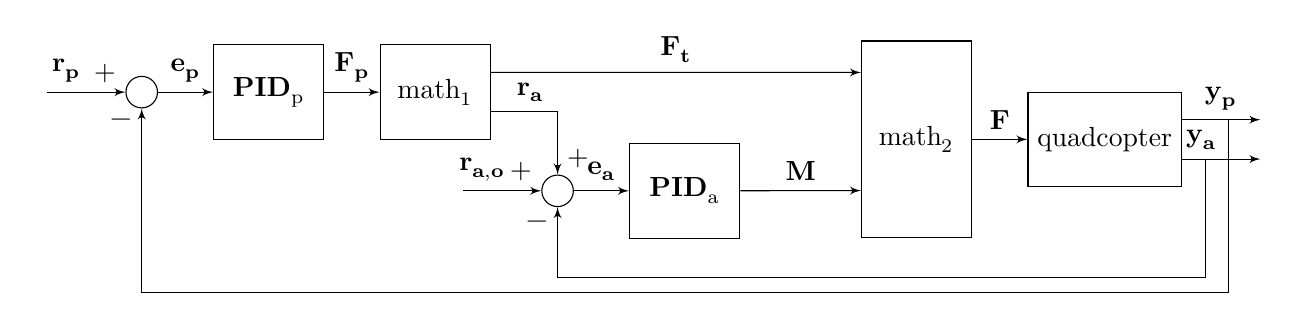
\begin{tikzpicture}[node distance=5mm and 7mm,>=latex']
	\node[io] (ref) {};
	\node[sum,right=1cm of ref] (sum1) {};
    \node[system,right=of sum1] (pid1) {\textbf{PID$_\mathrm{p}$}};
	\node[system,right=of pid1] (math1) {math$_1$};
	\node[sum,below right=of math1] (sum2) {};
	\node[io,left=1 cm of sum2] (refangle) {};
    \node[system,right=of sum2] (pid2) {\textbf{PID$_\mathrm{a}$}};
	\node[system,minimum height=25mm,right=of math1,xshift=40mm,yshift=-6mm]
      (math2) {math$_2$};
	\node[system,right=of math2] (quadcopter) {quadcopter};
    \node[io,right=1cm of quadcopter,yshift=+2.5mm] (pos) {};
    \node[io,right=1cm of quadcopter,yshift=-2.5mm] (rpy) {};

    \draw[->] (ref)  -- node[near start,above] {${\bf r_p}$} node[near end,above] {$+$} (sum1);
    \draw[->] (sum1) -- node[above] {${\bf e_p}$} (pid1);
    \draw[->] (pid1) -- node[above] {${\bf F_p}$} (math1);
    \draw[->] ($(math1.east)-(0,2.5mm)$) node[xshift=5mm,above]{${\bf r_a}$}
      -| node[very near end,right]{$+$} (sum2);
    \draw[->] (refangle) -- node[near start,above]{${\bf r_{a,o}}$}
      node[above,near end]{$+$} (sum2);
    \draw[->] (sum2) -- node[above]{${\bf e_a}$}(pid2);
    \draw[->] (pid2) -- node[above]{${\bf M}$}($(math2.west)-(0,6.5mm)$);
    \draw[->] (math2) -- node[above]{${\bf F}$}(quadcopter);
    \draw[->] ($(quadcopter.east)+(0,2.5mm)$) -- node[above]{${\bf y_p}$}(pos);
    \draw[->] ($(quadcopter.east)-(0,2.5mm)$) -- node[near start, above]{${\bf y_a}$}(rpy);
    \draw[->] ($(quadcopter.east)+(3mm,-2.5mm)$) -- ++(0,-15mm) -| node[very near end,left]{$-$} (sum2);
    \draw[->] ($(quadcopter.east)+(6mm,+2.5mm)$) -- ++(0,-22mm) -| node[very
      near end,yshift=4mm,left] {$-$}(sum1);
    \draw[->] ($(math1.east)+(0,2.5mm)$) -- node[above]{${\bf F_t}$} ($(math2.west)+(0,8.5mm)$);
\end{tikzpicture}
\caption{Blokschema voor de regeling van de quadcopter (zonder zwaartekracht en zwaartekrachtcompensatie).}
\label{fig:blokschema}
\end{figure}
Op het eerste gezicht ziet het blokschema er
nogal complex uit, maar de globale werking is toch vrij goed te doorgronden als
we er even wat langer bij stilstaan.
Wat allereerst opvalt, zijn twee terugkoppelkringen met
PID regelaars. Verder zien we blokken met math$_1$  en math$_2$, daar komen we
dadelijk nog op terug. En natuurlijk
weer de quadcopter.
De signalen zijn allemaal vetgedrukt, omdat we hier te maken hebben met
vectorsignalen, ofwel we hebben te maken met een multichannel systeem, ook wel
MIMO (multiple-input-multiple-output) genoemd. De referentie-ingang
$\mathbf{r_p}$  bestaat uit de referentie-waardes voor de positie (vandaar de
underscore p), dus voor de $x$-richting, de
$y$-richting en de $z$-richting, allemaal in het assenstelsel van de vaste
wereld, ofwel
\[
\mathbf{r_p} ~= ~ \left[\begin{array}{c}r_x\\ r_y \\ r_z\end{array}\right]
\]
Zo bestaat ook de uitgang $\mathbf{y_p}$ uit drie waardes, en wel de actuele
positie in de $x$-, de $y$- en de $z$-richting in het assenstelsel van de
vaste wereld, ofwel
\[
\mathbf{y_p}~ = ~ \left[\begin{array}{c}x\\y\\z\end{array}\right]
  \]
  De fout in de positie $\mathbf{e_p}$ is op vergelijkbare manier
  gedefinieerd. 
  
  Het blok \textbf{PID$_p$} bestaat dus uit drie PID regelaars,
  voor de $x$-, de $y$- en de $z$-richting. De uitgang is dan de vector
  $\mathbf{F_p}$ in $x$, $y$ en $z$-richting
  \[
  \mathbf{F_p}~ = ~ \left[\begin{array}{c}F_{p,x}\\ F_{p,y} \\ F_{p,z}\end{array}\right]
  \]
  met de kracht die we willen uitoefenen op de quadcopter. Als deze kracht
  $\mathbf{F_p}$ 
  loodrecht op het vlak van de quadcopter staat, dan is deze kracht de thrust
  $\mathbf{F}_t$ die we met de vier motoren kunnen uitoefenen. Maar heel vaak
  zal dat niet het geval zijn, en moeten we de quadcopter eerst kantelen
  voordat deze kracht loodrecht staat op het vlak van de quadcopter.

  De gewenste kantelhoek, zowel in de roll als in de pitch richting kunnen we
  echter berekenen. Deze berekening wordt gedaan in het blokje math$_1$ en is
  al geprogrammeerd in de voorbeeldcode. De wiskunde die hiervoor nodig is
maakt gebruik van
  Euler-hoeken en rotatie-matrices, voor nu gaat dat echter te ver (deze wordt
  behandeld in de minor Robotics and Vision Design). Wel moet je natuurlijk
  met het resultaat kunnen werken.

  Het eerste resultaat van math$_1$ is het deel van $\mathbf{F}_p$ wat al wel kan
  worden uitgevoerd door thrust van de quadcopter, ofwel $\mathbf{F_t}$ (om
  precies te zijn: de projectie van $\mathbf{F}_p$ op de lijn loodrecht op de
  quadcopter). Het tweede resultaat is de gewenste hoek $\mathbf{r_a}$ (de
  underscore a komt van het angle, het engelse woordt voor hoek). De vector
  $\mathbf{r_a}$ bestaat uit de gewenste \emph{roll}, \emph{pitch} en
  \emph{yaw}. De \emph{yaw} zullen we echter constant op 0 houden.

  Deze referentie hoek $\mathbf{r_a}$ is de referentie van een tweede set PID
  controllers, maar nu niet voor de positie, maar voor de orientatie van de
  quadcopter.

  Misschien is het je opgevallen, dat we nog een extra referentie-ingang
  hebben, namelijk $\mathbf{r_{a,o}}$. Deze extra ingang is niet nodig voor de
  autopilot, maar een handigheidje bij het tunen van de PID regelaar voor de
 roll en de pitch. Met behulp van $\mathbf{r_{a,o}}$ kunnen we zelf een
  setpoint waarde opgeven zodat we het effect van de roll en de pitch
  regelaars kunnen zien. Bijvoorbeeld als we de stapresponsie van de
  roll-controller willen zien, kiezen we 
  \[
  \mathbf{r_{a,o}} ~= ~ \left[\begin{array}{c}1\\0 \\0 \end{array}\right]
  \]
  En vervolgens kun je $\mathbf{r_{a,o}}$ bijvoorbeeld weer gelijk aan de 0-vector maken.

  De uitgang van de roll, pitch en yaw-controllers is het moment $\mathbf{M}$
  in de roll, pitch en yaw-richting. Het moment in de roll richting zorgt voor
  een hoekversnelling van de roll, ofwel rond de $x$-as van de quadcopter. Het
  moment in de roll richting kunnen we uitoefenen door middel van een koppel
  dat gegenereerd wordt door de 2 motoren op de $y$-as van de quadcopter. Op
  dezelfde manier kan het moment in de pitch richting worden uitgeoefend door
  middel van een koppel dat gegenereerd wordt door de 2 motoren op de $x$-as
  van de quadcopter. Het moment in de yaw-richting zal niet met behulp van de
  4 motoren worden uitgeoefend, aangezien we uitgaan van de versimpelde
    situatie dat de motoren krachtactuatoren zijn. De yaw zal direct worden
    doorgegeven aan de \textbf{pybullet} module om een moment uit te oefenen
    op de quadcopter in de yaw-richting, ofwel langs de $z$-as van de
    quadcopter (NB Dit wordt niet weergegeven in het blokschema van
    Figuur~\ref{fig:blokschema}!).

    Het omrekenen van de thrust $\mathbf{F_t}$ en de momenten  in de roll en
    de pitch richting (eerste twee elementen in $\mathbf{M}$) wordt gedaan in
    het blokje math$_2$. Dit omrekenen gaat vrij eenvoudig, en komt in wezen
    neer op het omrekenen van de momenten in koppels en het sommeren van de
    krachten, en is ook reeds ge\"implementeerd in de voorbeeldcode.
    Het resultaat is de vector $\mathbf{F}$ die bestaat uit de 4 krachten voor
    elke actuator \'e\'en.

    De actuatorkrachten $\mathbf{F}$ worden doorgegeven aan de
    \texttt{pybullet} module die de simulatie van de quadcopter uitvoert. Het
    resultaat is een positie-vector $\mathbf{y_p}$ en een ori\"entatie-vector
    $\mathbf{y_a}$, met daarin de roll, pitch en yaw.

    De \texttt{pybullet} module geeft echter niet direct de ori\"entatie in
    termen van roll, pitch en yaw, maar in termen van een \emph{quaternion}.
    Quaternions zijn een uitbreiding op complexe getallen, en 
    door de Ierse wiskunde William Rowan Hamilton ge\"introduceerd, zie
    bijvoorbeeld de Wiki \url{https://nl.wikipedia.org/wiki/Quaternion}. Lange tijd
    waren quaternions alleen interessant voor wiskundigen, maar tegenwoordig worden quaternions veel gebruikt in robotica en computergraphics, zelfs de meeste grafische kaarten kunnen tegenwoordig rekenen met quaternions. Voor nu is het voldoende te bedenken dat een quaternion bestaat uit vier re\"eele getallen die samen een ori\"entatie defini\"eren en eenvoudig omgerekend kunnen worden naar drie Euler hoeken, ofwel roll, pitch en yaw. Dat laatste wordt gedaan in de \texttt{pybullet}-functie \texttt{getEulerFromQuaternion}, daar hoeven we ons dus niet meer druk over te maken.

\section{Uitleg van \texttt{quadcopter\_sim.py}}
\label{sec:implementatie}
Zie de documentatie in het voorbeeld \texttt{quadcopter\_sim.py} en het overzicht van de variabelen in Tabel~\ref{tab:symbol}. 
\begin{table}
\caption{Overzicht van de symbolen uit het blokschema van Figuur~\ref{fig:blokschema} met de bijbehorende variabele in de Python simulatie en hun omschrijving.}
\label{tab:symbol}
  \centering
  \begin{tabular}{lll}
    \hline\hline
    Symbool & Variabele & Omschrijving \\
    \hline
    ${\bf r_p}$ & \texttt{ref\_pos} & Referentie positie (x/y/z) op te geven
    door gebruiker (3D vector)\\
    ${\bf r_a}$ & \texttt{ref\_rpy} & Referentie hoek (roll/pitch/yaw) berekend op basis van ${\bf F_p}$ (3D vector)\\
    ${\bf r_{a,o}}$ & \texttt{ref\_rpy\_offset} & Referentie hoek
    (roll/pitch/yaw) op te geven door gebruiker (3D vector)\\
    && (NB: wordt alleen gebruikt ten behoeve van instellen \textbf{PID$_a$}
    (roll/pitch/\\
    &&    yaw) regelaars!)\\
    ${\bf y_p}$ & \texttt{pos\_meas} & Positie  (x/y/z) van de quadcopter (3D vector)\\
    ${\bf y_a}$ & \texttt{rpy\_meas} & Hoek (roll/pitch/yaw) van de quadcopter (3D vector)\\
    ${\bf e_p}$ & \texttt{error\_pos} & Resterende fout in positie (x/y/z) (3D vector)\\
    ${\bf e_a}$ & \texttt{error\_rpy} & Resterende fout in hoek (roll/pitch/yaw) (3D vector)\\
    \textbf{PID$_p$} & \texttt{x\_ctrl} & 3 PID controllers voor positie
    regeling (x/y/z) \\
      & \texttt{y\_ctrl} & \\
      & \texttt{z\_ctrl} & \\
    \textbf{PID$_a$} & \texttt{roll\_ctrl} & 3 PID controllers voor hoek
    (roll/pitch/yaw) regeling \\
      & \texttt{pitch\_ctrl} & \\
      & \texttt{yaw\_ctrl} & \\
    ${\bf F_p}$ & \texttt{force\_pos} & Kracht om naar gewenste positie ${\bf
    r_p}$ te
    sturen (3D vector)\\
    ${\bf F_t}$ & \texttt{thrust} & Hoeveelheid kracht loodrecht op vlak van
    de quadcopter, is gelijk aan \\
     && som van de 4 motorkrachten  (3D vector)\\
    ${\bf F}$ & \texttt{force\_act1..4} & Vector met de 4 actuatorkrachten 
     (4D vector)\\
     ${\bf M}$ & \texttt{moments} & Momenten om naar gewenste hoek ${\bf
     r_a}+{\bf r_{a,o}}$ te sturen
       (3D vector)\\
       math$_1$ & & formules om de thrust ${\bf F_t}$ en de benodigde hoek
       ${\bf r_a}$ te berekenen\\
       math$_2$ & & formules om op basis van de thrust ${\bf F_t}$ en de
       momenten ${\bf M}$ de 4 \\
         && actuatorkrachten ${\bf F}$ te berekenen \\
      quadcopter && simulatie van de quadcopter met behulp van de
      \texttt{pybullet} module\\
\hline\hline
  \end{tabular}

\end{table}
Verder bedenk dat de quadcopter controller een object is, genaamd \texttt{qcc}. Objecten bevatten doorgaans data, dat kunnen ook andere objecten zijn, en methodes (of functies). Data kunnen we zowel lezen als schrijven. In het volgende voorbeeld bekijken we eerst de waarde van de referentie-positie \texttt{ref\_pos}, daarna veranderen we deze in de vector $\left[0,0,2\right]$, bekijken deze opnieuw en bekijken vervolgens ook de waarde van \texttt{error\_pos}
\begin{verbatim}
>>> qcc.ref_pos
>>> qcc.ref_pos = np.array([0,0,2])
>>> qcc.ref_pos
>>> qcc.error_pos
\end{verbatim}
Ook de gains van de PID controllers kunnen we op deze manier opvragen en aanpassen. Bijvoorbeeld voor de $z$-controller:
\begin{verbatim}
>>> qcc.z_ctrl.Kp
>>> qcc.z_ctrl.Kp = 5
>>> qcc.z_ctrl.Kp
>>> qcc.z_ctrl.Ki
>>> qcc.z_ctrl.Ki = 0
>>> qcc.z_ctrl.Kd
>>> qcc.z_ctrl.Kd = 1
\end{verbatim}
Voor de andere controllers gaat dit op dezelfde manier. 

Als je onbekend bent met object ge\"orienteerd programmeren in Python, dan is
het aan te raden een korte introductie zoals
\url{https://nl.wikibooks.org/wiki/Programmeren_in_Python/Object-georiënteerd_programmeren}
door te nemen. Ook op youtube staan nuttige filmpjes met uitleg over object
georienteerd programmeren in Python, bijv.\ die van Derek Banas
\url{https://www.youtube.com/watch?v=1AGyBuVCTeE}.

\section{Opdracht tutorial UAVREG}
\label{sec:opdracht}
\subsection{Stappen}
\subsubsection{Stap 0: Bestudeer deze handout en voorbeeld code}
\subsubsection{Stap 1: PID-regelaar implementatie}
Ga na hoe je een PID controller kunt implementeren en pas de code in
\texttt{quadcopter\_sim.py} aan.
 
\subsubsection{Stap 2: Hoogte ($z$) regeling}
\label{sec:hoogte}
Ga na hoe je de zwaartekracht kan compenseren en tune de PID controller voor de $z$-richting. Tip: begin met $K_p$, vervolgens $K_d$ en evt.\ $K_i$.

\subsubsection{Stap 3: Roll/pitch regeling (yaw is al gedaan)}
\label{sec:rollpitch}
Tune de Roll en de Pitch controllers. Vanwege symmetrie in de quadcopter kun je voor de pitch regeling dezelfde controller parameters gebruiken als de roll-richting. Hint: Gebruik de offset op de referentie \texttt{qcc.ref\_rpy\_offset} en zet gravity volledig uit (\texttt{p.setGravity(0,0,0)}) tijdens het tunen van deze regelaars zodat de quadcopter niet `wegloopt'  als deze wordt geroteerd.
Zorg ervoor dat de roll en de pitch regelingen `voldoende snel' zijn ten opzichte van de positie regeling. De positieregeling gaat er namelijk vanuit dat de stand van de quadcopter namelijk correct wordt aangenomen. 

\subsubsection{Stap 4: Horizontale ($x$/$y$) regeling}
\label{sec:horizontaal}
Ook hier geldt weer, begin met $K_p$, dan $K_d$ en evt.\ nog $K_i$. Vanwege symmetrie kun je voor de $y$-regelaar dezelfde waarden kiezen als in de $x$-richting. 

\subsection{Afteken opdracht: Baan-regeling}
Bedenk een baan bestaande uit ten minste 10 punten in de 3D ruimte (mag ook meer, ook veel meer). Leg deze baan af met de quadcopter autopilot die je zojuist hebt geprogrammeerd. Denk na over de snelheid waarmee de baan wordt doorlopen.
Demonstreer je baanregeling en zorg dat je je code en de keuze van de PID parameters kunt uitleggen.

% Erwin Coumans
% pybullet quickstart guide
% 2017
% Online
% https://docs.google.com/document/d/10sXEhzFRSnvFcl3XxNGhnD4N2SedqwdAvK3dsihxVUA/edit?usp=sharing



\end{document}
